\section{数据集、评价指标与方法方案}\label{sec:method}

\subsection{实验基础}

本章介绍数据集来源、预处理方式、评价指标、模型选择和实验口径，为实验结果分析与系统实现提供统一基础。

\subsection{数据集介绍}

本文的实验统一采用 LEVIR-Ship 数据集\cite{chen2022_tinyship_drenet}。该数据集主要面向中分辨率遥感微小船舶检测任务，在复杂海面背景下能够较好反映小目标检出的实际难点，数据集划分如表~\ref{tab:ch3_dataset_split}所示。

\begin{table}[htbp]
  \centering
  \caption{LEVIR-Ship 数据集划分}
  \label{tab:ch3_dataset_split}
  \begin{tabular}{lcc}
    \toprule
    数据子集 & 图像数量 & 目标数量 \\
    \midrule
    训练集 & 2321 & 2002 \\
    验证集 & 788 & 665 \\
    测试集 & 788 & 552 \\
    \bottomrule
  \end{tabular}
\end{table}

LEVIR-Ship 中船舶目标普遍较小，背景纹理较为复杂。部分图像中，船体与海浪、岸线或港区设施之间的纹理差异有限，后处理阈值的变化会直接影响模型输出。基于这一特点，本文在实验设计中并未仅以单一主指标评价模型优劣，而是同时记录检出能力、误检控制和工程部署相关指标。

\subsection{数据集样例与任务特征}

LEVIR-Ship 涵盖了开阔海域、近岸区域、港口区域和多目标密集分布等场景，不同图像块之间背景纹理、目标密度、朝向和局部对比度的差异较大。模型一方面要对微弱目标保持敏感，另一方面又要抑制复杂背景中的伪目标响应。“目标小而背景强”这一矛盾构成了遥感微小船舶检测的核心难点。

\begin{figure}[htbp]
  \centering
  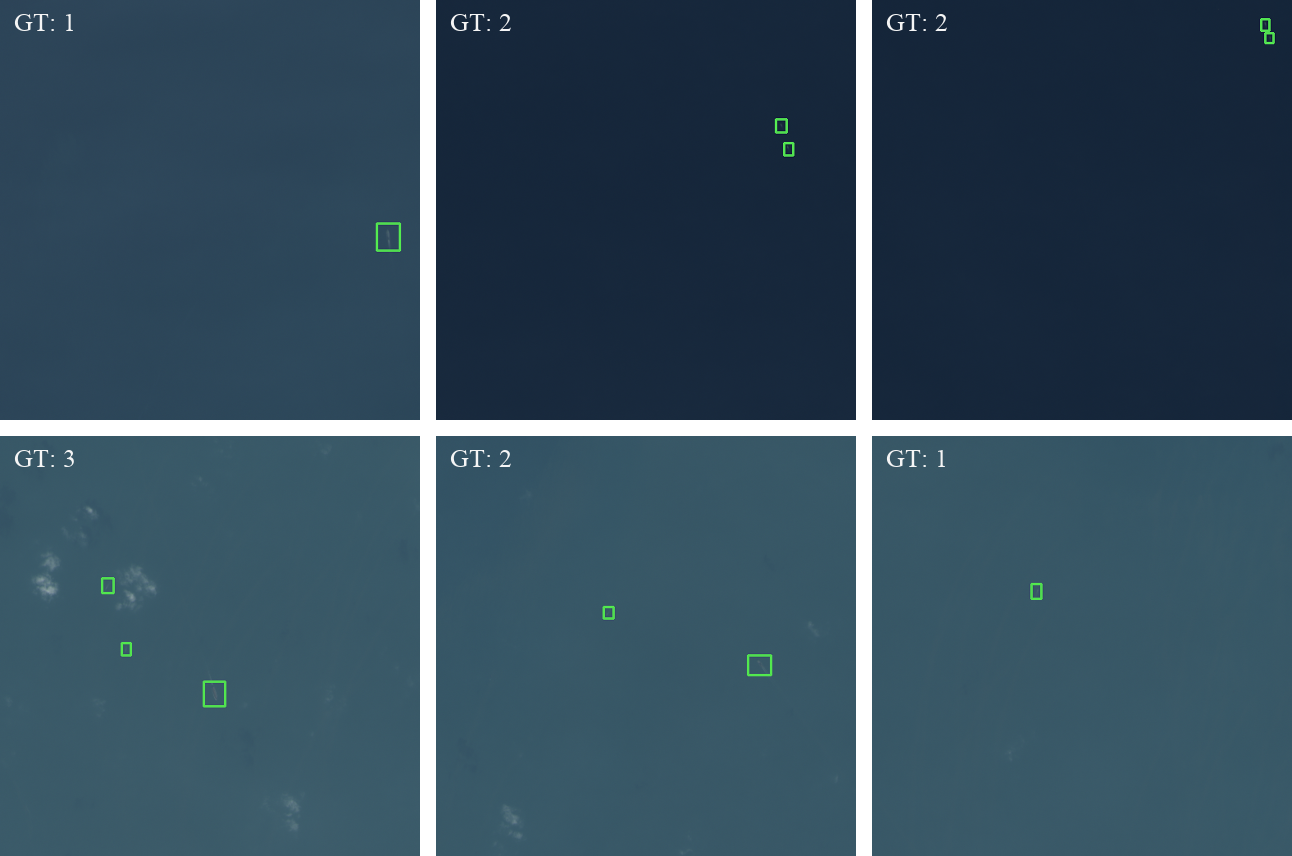
\includegraphics[width=\textwidth]{img/ch3_dataset_examples.png}
  \caption{LEVIR-Ship 数据集典型样例}
  \label{fig:ch3_dataset_examples}
\end{figure}

图~\ref{fig:ch3_dataset_examples} 展示了不同场景的样例图像。除 AP50 外，本文还记录精度、召回率和 F1 值，并保留成功检测、漏检和误检样例，以观察模型在不同背景条件下的具体表现。

\subsection{数据预处理与统一格式}

在跨框架实验中，较易产生偏差的环节往往是数据和评测脚本，而非网络结构本身。因此，为减小这部分误差，实验前先统一数据预处理和结果组织方式。

本文首先核对图像与标注文件是否一一对应，并检查空标注、异常坐标和类别不一致等情况；随后将数据统一整理为 COCO 中间格式，使 MMDetection 路线和 YOLO 路线尽量共用同一套评测基础；在此基础上固定 train、val、test 划分及样本清单，以避免模型之间因样本范围不同而产生额外差异；最后，将各模型输出统一整理为包含 \texttt{image\_id}、\texttt{model\_name}、\texttt{bbox}、\texttt{score} 和 \texttt{category\_id} 的结构化记录，供可视化和数据库存储使用。

通过上述处理方式，本文实现了跨模型的数据组织、评测口径与结果表达统一，使模型差异尽可能反映检测范式和实现策略本身，而非数据划分、评测脚本或输出字段设置的不一致。统一格式和统一口径因此构成了本文实验方法的重要组成部分，并为后续结果比较与解释提供了基础。

统一格式也直接服务于系统实现。不同框架与实现方式的推理结果可以进入同一套后处理与可视化逻辑；结构化结果也能写入 Web 系统数据库，使离线实验结果和在线任务回放使用同一类数据表达。数据预处理与统一格式流程如图~\ref{fig:ch3_preprocess_flow}所示。

\begin{figure}[htbp]
  \centering
  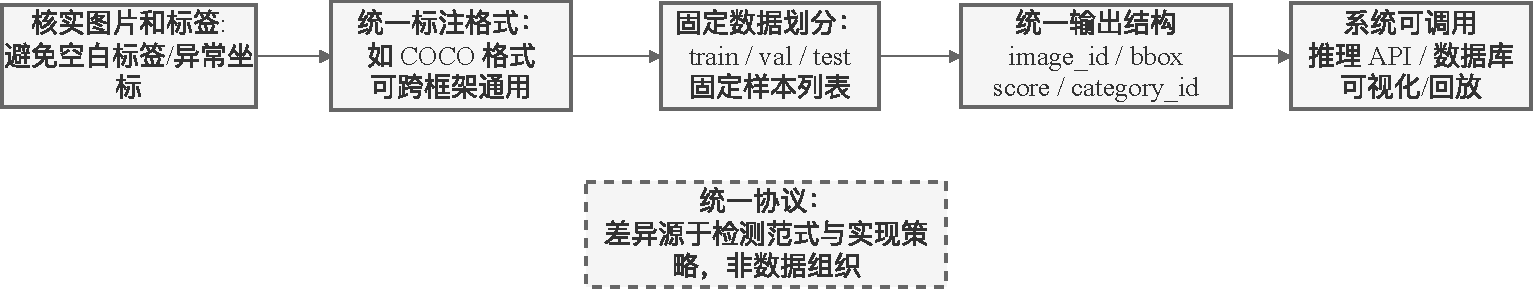
\includegraphics[width=\textwidth]{img2_pdf/ch3_preprocess_flow.pdf}
  \caption{数据预处理与统一格式流程图}
  \label{fig:ch3_preprocess_flow}
\end{figure}

\subsection{评价指标}

本文实验使用 AP50 作为主指标，AP50-95、精度、召回率与 F1 值作为辅助指标，其相关定义如下：

\begin{equation}
\text{Precision} = \frac{TP}{TP + FP}\text{,}
\end{equation}

\begin{equation}
\text{Recall} = \frac{TP}{TP + FN}\text{,}
\end{equation}

\begin{equation}
F1 = \frac{2 \cdot \text{Precision} \cdot \text{Recall}}{\text{Precision} + \text{Recall}}\text{,}
\end{equation}

\begin{equation}
\text{IoU} = \frac{|B_{pred} \cap B_{gt}|}{|B_{pred} \cup B_{gt}|}\text{.}
\end{equation}

其中，精度（Precision）用于反映预测结果中真正例所占比例，召回率（Recall）用于反映真实目标被检出的比例，F1 值用于综合衡量精度与召回率之间的平衡，交并比（IoU）用于衡量预测框与标注框之间的重叠程度。AP50 对应交并比（IoU）阈值为 0.5 时的平均精度，本文用其观察模型能否有效检出微小船舶；AP50-95 覆盖多个交并比阈值，对边框位置质量更敏感；精度更接近误检控制情况，召回率更接近漏检控制情况，F1 值用于观察二者折中。本文还记录帧率（FPS）、参数量和 FLOPs 等效率指标，用于讨论模型接入系统时的部署成本。相关评测口径与交并比阈值区间设置与 COCO 指标定义保持一致\cite{lin2014_coco}。

\subsection{指标选择依据}

本文将 AP50 设为主评价指标，主要是考虑到遥感图像中的船舶目标尺度较小，预测框和标注框只要偏移几个像素，交并比就可能明显变化。若过度依赖高交并比阈值，边框回归误差会被放大，模型是否完成有效检出反而不易判断。故 AP50 用于衡量基本检出能力，AP50-95 则补充反映定位质量。

精度、召回率和 F1 值在本文中同样重要。由于 DRENet、FCOS 与 YOLO26 的设计出发点不同，若仅按照 AP50 排序，容易掩盖误检与漏检之间的取舍差异。召回率较高的模型更适合目标排查类场景，精度较高的模型则更适合结果输出需要稳定可控的系统展示场景。因此，精度与召回率平衡也是本文解释模型行为的重要依据。

\subsection{模型方案}

为了让对比不局限在同一类检测器内部，本文选取三类模型：DRENet 对应遥感微小船舶专项方法，FCOS 对应无锚框检测路线，YOLO26 对应单阶段检测路线。

\subsubsection{遥感微小船舶检测专用方法：DRENet}

DRENet 是针对 LEVIR-Ship 数据集提出的专项方法\cite{chen2022_tinyship_drenet}。该方法在训练阶段引入退化重建增强机制，目的是加强网络对弱纹理船舶目标的辨识能力。如图~\ref{fig:ch3_drenet_flow}为 DRENet 的检测流程：训练阶段由增强路径与检测主干共同参与特征学习，推理阶段则仅保留检测主干完成目标检出。

\begin{figure}[htbp]
  \centering
  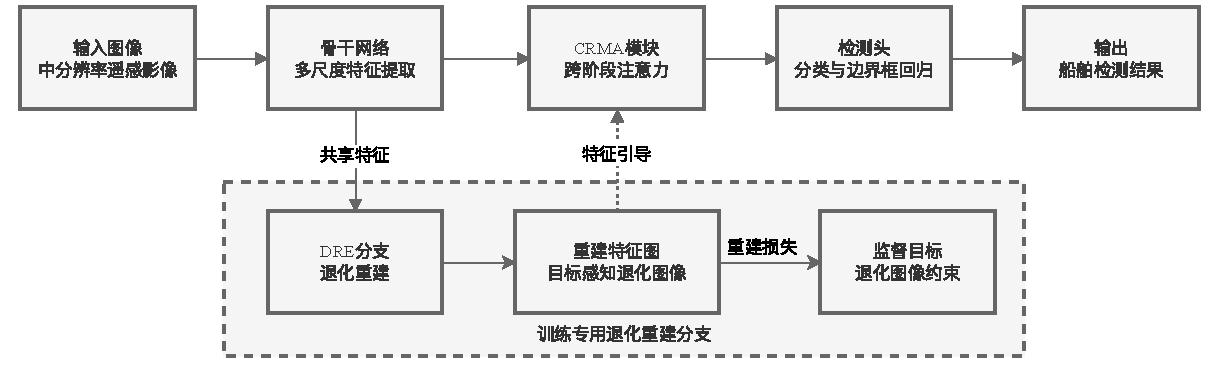
\includegraphics[width=\textwidth]{img2_pdf/ch3_drenet_overview.pdf}
  \caption{DRENet 检测流程示意}
  \label{fig:ch3_drenet_flow}
\end{figure}

从网络结构看，DRENet 由检测主干路径和训练期增强路径两部分组成。检测主干负责常规定位与分类，增强路径则借助退化重建任务向骨干特征补充弱纹理目标的判别信息，并在训练阶段提供附加监督。经此处理后，模型对微小、低对比船舶的响应能力会有所增强。

DRENet 的主要设计特点包括以下三点：

\begin{enumerate}[label=（\arabic*）, leftmargin=3.5em]
  \item \textbf{退化重建增强机制}：训练阶段先对输入图像施加模糊、噪声和分辨率下降等模拟退化，再要求网络从退化后的图像中重建原始外观。该辅助分支与检测主干共享同一骨干网络，因此骨干特征同时受到检测损失与重建损失约束，有助于加强模型对弱纹理目标的判别能力。
  \item \textbf{跨阶段区域记忆增强模块（CRMA）}：该模块将保留空间细节与边缘信息的浅层特征，与承载语义判别信息的深层特征进行跨阶段连接和融合，使小目标的定位线索在下采样过程中不易被削弱。与仅依赖特征金字塔网络（FPN）自顶向下传播的方式相比，CRMA 提供了更直接的浅层与深层协同通道。
  \item \textbf{双路径联合训练策略}：检测路径与重建路径在训练期间并行运行，推理阶段只保留检测路径，因此不会额外增加推理开销。该设计既保留了训练阶段的增强约束，也兼顾了部署阶段的计算效率。

\end{enumerate}

后续实验结果表明，DRENet 通常具有较高的召回率，但在复杂背景下也更容易产生误检。因此该方法更适合用于召回优先的检测场景。DRENet 的网络结构如图~\ref{fig:ch3_drenet_overview} 所示，其核心在于将退化重建增强分支与检测主干协同训练，以提高对弱纹理目标的敏感性。

\begin{figure}[htbp]
  \centering
  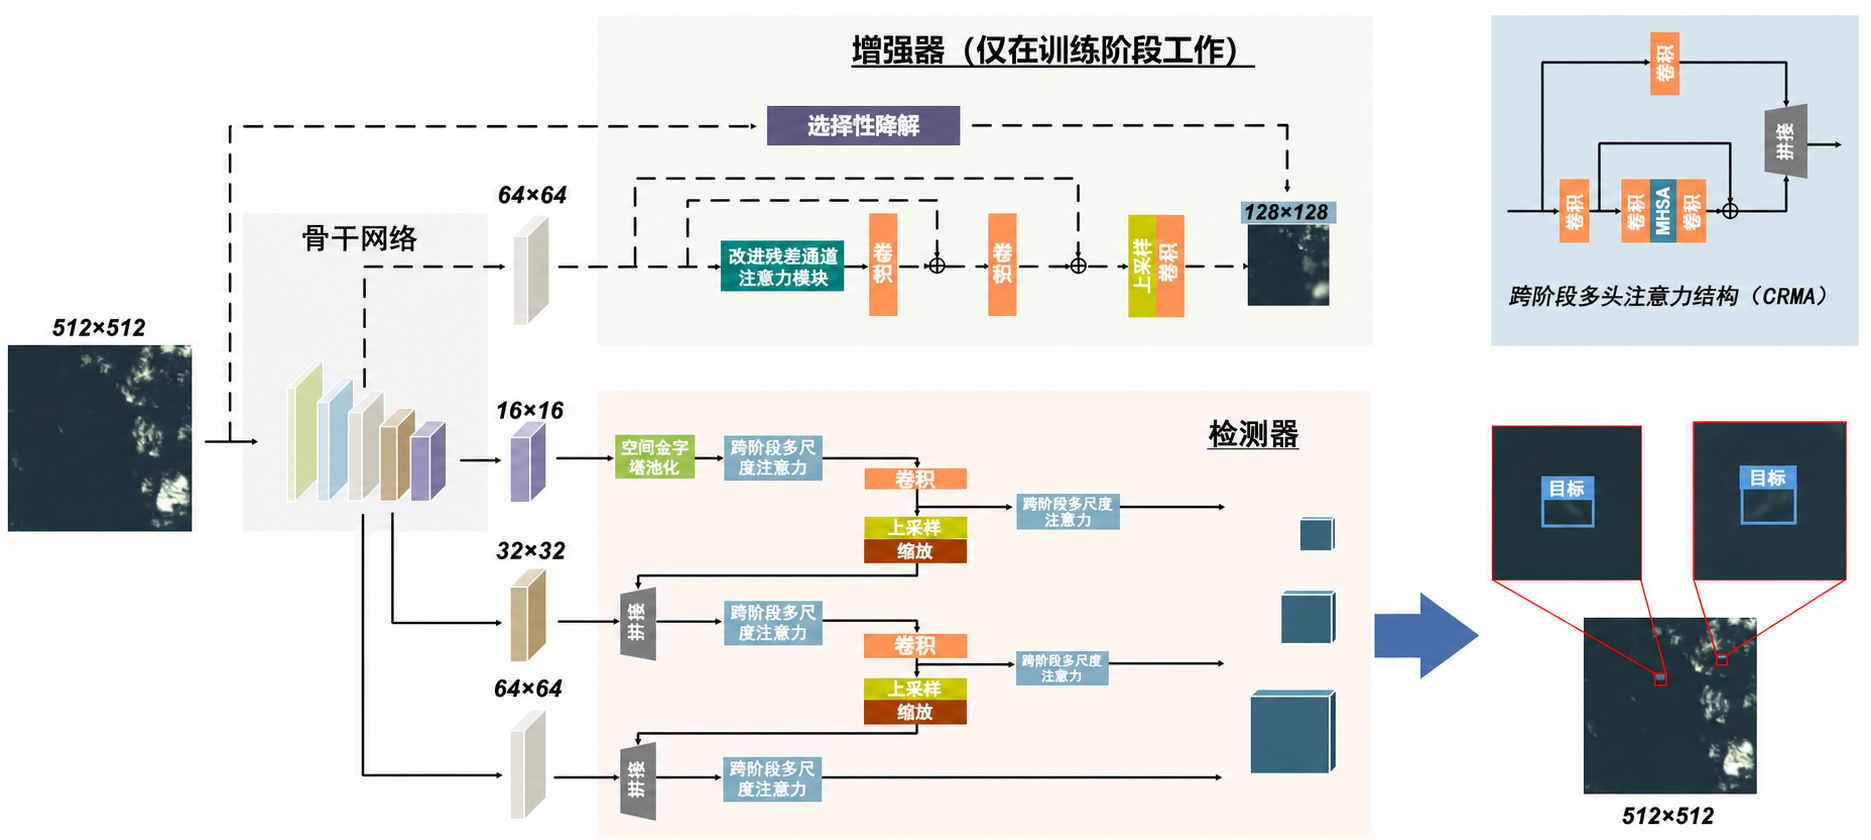
\includegraphics[width=\textwidth]{img/ch3_drenet_network_from_paper.png}
  \caption{DRENet 网络结构图，引自\cite{chen2022_tinyship_drenet}}
  \label{fig:ch3_drenet_overview}
\end{figure}

\subsubsection{无锚框代表性目标检测方法：FCOS}

FCOS 用位置回归替代锚框设计，减少了对锚框尺寸、比例和匹配策略等超参数的依赖\cite{tian2019_fcos}。本文将其作为无锚框路线的代表模型，与专项方法和单阶段路线置于同一评测口径下比较，以考察该类方法在遥感微小船舶任务中的实际表现。图~\ref{fig:ch3_fcos_flow} 展示了 FCOS 的检测流程：模型在多尺度特征图上直接进行逐点回归，并结合中心概率分支完成候选框排序与筛选。

\begin{figure}[htbp]
  \centering
  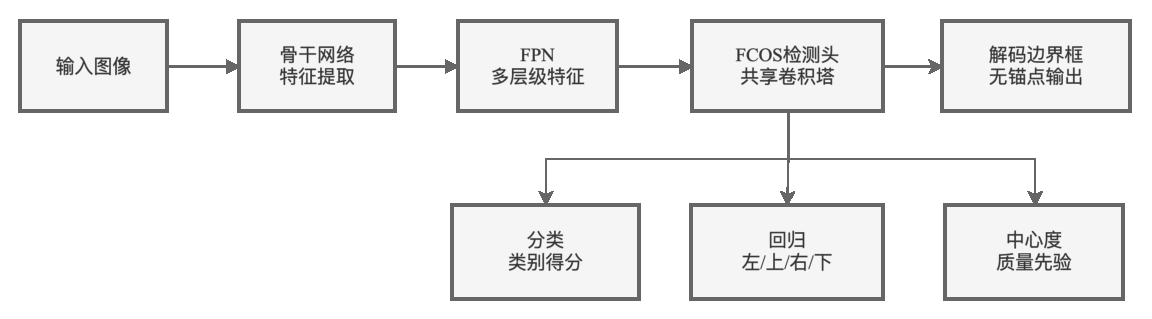
\includegraphics[width=\textwidth]{img2_pdf/ch3_fcos_pipeline.pdf}
  \caption{FCOS 检测流程示意}
  \label{fig:ch3_fcos_flow}
\end{figure}

FCOS 的基本机理是无锚框密集回归，输入图像经主干网络与特征金字塔网络（FPN）生成多尺度特征后，检测头在每个位置直接预测边框偏移和类别分数，并通过中心概率分支评估预测质量，随后由分类分数与中心概率联合排序，再经非极大值抑制（NMS）输出检测结果。

FCOS 的主要设计特点包括以下三点：

\begin{enumerate}[label=（\arabic*）, leftmargin=3.5em]

  \item \textbf{逐点预测替代锚框匹配}：FCOS 在特征图每个位置直接预测该点到目标边界框四条边的距离偏移（上、下、左、右）以及类别概率，完全取消了锚框的尺度、比例和匹配阈值等超参数设计。该设计既降低了跨数据集迁移时的调参负担，也避免了锚框匹配中正负样本定义不一致的问题。
  \item \textbf{中心概率分支抑制低质量候选}：远离目标中心的特征点更容易产生定位不准确的预测框，这类低质量候选会削弱整体排序效果。为此 FCOS 引入中心概率分支，预测每个点距目标中心的相对距离，并将中心概率与分类分数相乘作为最终排序依据，从而抑制边缘区域的低质量候选框，提升检测结果的排序稳定性。
  \item \textbf{基于 FPN 层级的尺度分配策略}：FCOS 为不同 FPN 层级显式指定目标尺度范围，使每个层级只负责特定大小区间的目标检测。该设计可以减少不同层级之间的预测重叠与竞争，并使小目标在浅层层级获得更充分的响应空间。

\end{enumerate}

在本课题中，FCOS 的精度与召回率折中相对稳定，但对输入尺寸较为敏感，当推理输入过小时，特征图分辨率不足以支撑逐点回归精度。FCOS 的网络结构如图~\ref{fig:ch3_fcos_pipeline} 所示，其主干网络、特征金字塔网络和检测头共同构成了典型的无锚框检测框架。

\begin{figure}[H]
  \centering
  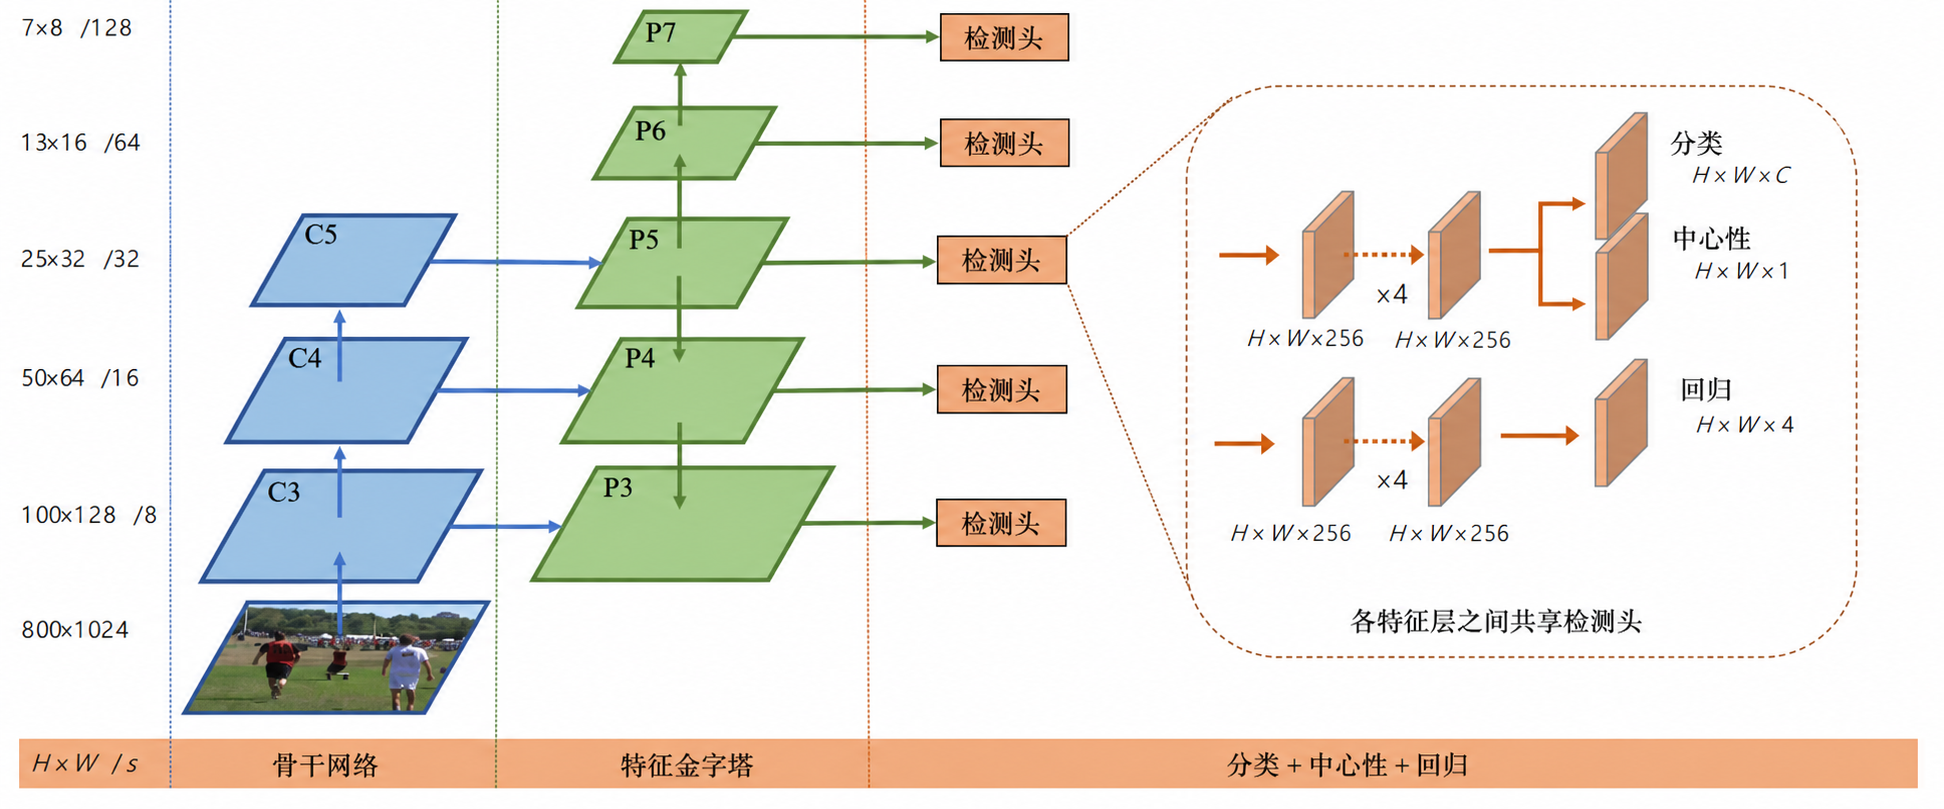
\includegraphics[width=\textwidth]{img/ch3_fcos_network_from_paper.png}
  \caption{FCOS 网络结构图，引自\cite{tian2019_fcos}}
  \label{fig:ch3_fcos_pipeline}
\end{figure}

\subsubsection{单阶段代表性目标检测方法：YOLO26}

YOLO 系列以单阶段预测和推理效率见长，在工程部署中使用较多\cite{redmon2016_yolo,redmon2018_yolov3}。本文选取 YOLO26 代表单阶段路线，主要考察其在检测精度、边框质量、训练链路成熟度和系统接入成本之间的表现。图~\ref{fig:ch3_yolo_flow} 展示了 YOLO26 的检测流程，即通过主干网络提取特征、特征融合层进行跨尺度融合，并由多尺度检测头完成目标预测。

\begin{figure}[H]
  \centering
  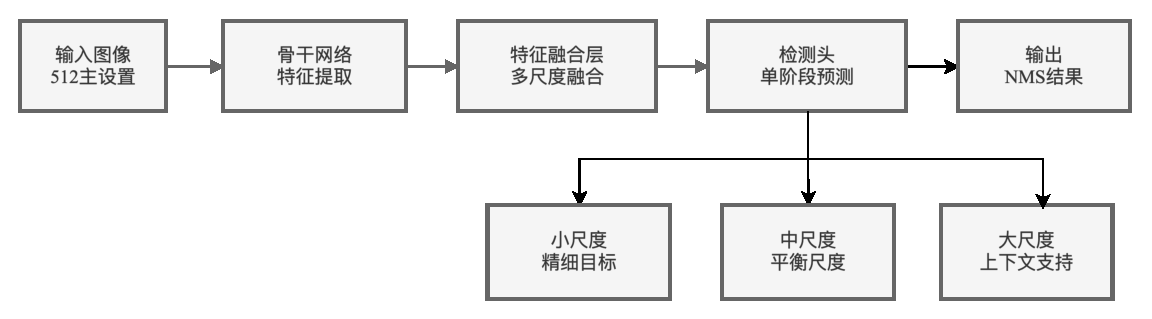
\includegraphics[width=\textwidth]{img2_pdf/ch3_yolo_pipeline.pdf}
  \caption{YOLO26 检测流程示意}
  \label{fig:ch3_yolo_flow}
\end{figure}

YOLO26 延续单阶段端到端范式。主干网络负责提取语义特征，特征融合层执行跨尺度融合，检测头在多个尺度上同时输出候选框与类别分数，单次前向即可完成检出。该结构在工程部署中具有较好的吞吐效率。

YOLO 路线的主要设计特点包括以下三点：

\begin{enumerate}[label=（\arabic*）, leftmargin=3.5em]
  \item \textbf{多尺度检测头增强小目标可见性}：YOLO26 在三个不同尺度的特征图（P3、P4、P5）上同时设置检测头。由于浅层特征图分辨率较高，模型能够保留更多小目标细节信息，因此微小船舶在浅层层级可以获得更充分的候选框生成机会。与只在单一尺度输出的检测器相比，多尺度检测头对小目标的覆盖更完整。
  \item \textbf{结构轻量化与高效模块设计}：YOLO26 采用 C2f 等高效构建模块替代传统重参数卷积，在保持特征表达能力的同时控制参数量与计算量。本文实验中，YOLO26 的参数量为 2.5M、FLOPs 为 3.7G，明显低于 FCOS 的 32.2M 与 123.0G，因此在部署场景中具有更高的吞吐效率。
  \item \textbf{任务对齐分配与训练增强策略}：YOLO26 采用任务对齐分配替代传统交并比匹配策略，将分类质量与定位质量联合用于正负样本分配，使训练阶段的样本定义更贴近最终评测目标。同时配合 Mosaic、MixUp 等数据增强策略，可提升模型对稀疏小目标和复杂背景的泛化能力。

\end{enumerate}

在本课题中，YOLO26 的输出结果较为稳定，部署链路也更成熟，因此适合作为系统中的默认候选方案。与 DRENet 相比，YOLO26 在误检控制方面更为稳定，两者在模型行为上也具有一定互补性。YOLO26 的网络结构如图~\ref{fig:ch3_yolo_pipeline} 所示，该结构通过轻量化模块与多尺度检测头兼顾检测精度和部署效率。

\begin{figure}[htbp]
  \centering
  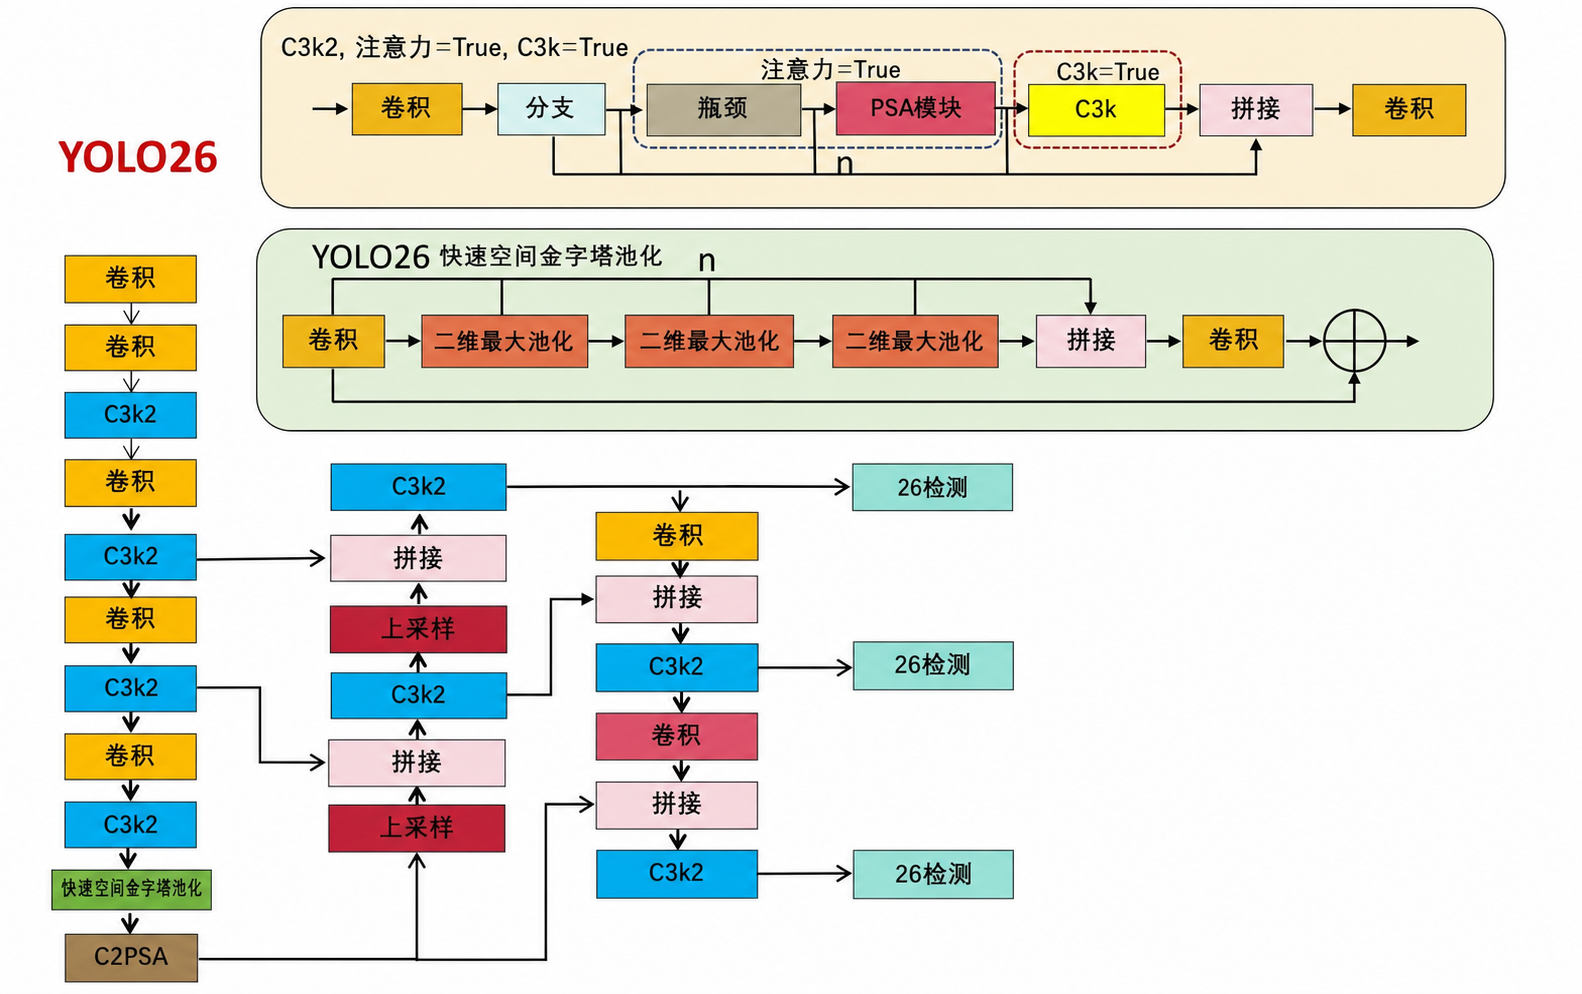
\includegraphics[width=\textwidth]{img/ch3_yolo_network_from_paper.png}
  \caption{YOLO26 网络结构图，引自\cite{redmon2018_yolov3}}
  \label{fig:ch3_yolo_pipeline}
\end{figure}

\subsection{统一实验协议与实现约束}

本文对实验协议作出统一约束：数据划分和评测口径保持一致，实验环境、配置文件、权重路径、日志文件和关键结果均保留记录，结果输出结构也作统一整理，以便系统侧调用。统一协议并不意味着将所有模型改造成完全相同的实现形式，而是在保留各自实现特征的前提下，采用统一评测流程比较不同模型在同一任务中的表现。

在实现层面，本文通过统一推理入口封装不同模型能力：

\texttt{predict(image\_path, model\_name, conf\_threshold, iou\_threshold)}

在统一推理入口基础上，本文进一步封装了融合推理接口和系统任务执行逻辑，模型训练后的离线评测、命令行单图推理、批量推理以及 Web 系统接入，均调用同一个核心入口。

\subsection{本章总结}

本章围绕实验基础与方法方案，对比较研究所需的数据、指标和模型设置进行了统一说明。文中介绍了 LEVIR-Ship 数据集的任务特点、数据预处理与结构化记录方式，明确了 AP50、AP50-95、精度、召回率和 F1 值等评价指标及其选择依据，并说明了 DRENet、FCOS 和 YOLO26 三类代表模型的设计特点、选取原因以及统一实验协议和推理接口封装约束。这些内容为第四章的实验结果分析和第五章的系统接入实现提供了统一基础。
